\documentclass[sigconf,review]{acmart}

\usepackage{amsmath,amssymb,amsfonts,latexsym}
\usepackage{enumerate}
\usepackage{xspace}
\usepackage{epsf,picinpar}
\usepackage{varioref}
\usepackage{colortbl,multirow,hhline}
\usepackage{listings}
\usepackage{amssymb}
\usepackage{colortbl,multirow,hhline}
\usepackage{algorithmic}
\usepackage{algorithm}
\usepackage{caption}
\usepackage[normalem]{ulem}
\usepackage{xcolor}
\usepackage{pifont}
\usepackage{xcolor,colortbl}
\usepackage{url}
\usepackage{balance}
\usepackage{graphicx, subfigure}
\usepackage{longtable}
\usepackage{lscape}
\usepackage{multirow}
\usepackage{listings}
\usepackage{framed}
\usepackage{morefloats}
\usepackage[T1]{fontenc}
\usepackage{array}
\usepackage{pdfpages}
\usepackage{fancybox}
\usepackage{amsmath}
\usepackage{flushend}
\usepackage{booktabs}
\usepackage{enumitem}
\usepackage{makecell}
\usepackage{hyperref}
\usepackage{threeparttable}
\usepackage{bm}
\renewcommand{\ttdefault}{cmr}

%\newcommand{\limit}[1]{\textcolor{red}{\noindent \ding{46}~Page limit:~#1}\\}
\newcommand{\todo}[1]{\textcolor{blue}{\ding{46}~#1}} 
\newcommand{\ie}{\emph{i.e.,}\xspace}
\newcommand{\eg}{\emph{e.g.,}\xspace}
\newcommand{\etc}{etc.\xspace}
\newcommand{\etal}{\emph{et~al.}\xspace} 

\copyrightyear{2022}
\acmYear{2022}
\setcopyright{acmcopyright}
\acmConference[Green Lab 2022/2023]{Green Lab 2022/2023 - Vrije Universiteit Amsterdam}{September--October, 2022}{Amsterdam, The Netherlands}
\acmBooktitle{Green Lab 2022/2023 - Vrije Universiteit Amsterdam, September--October, 2022, Amsterdam (The Netherlands)}
  
\begin{document}

\title{
	Energy Consumption on Music Players:\\
 An Empirical Analysis on Spotify and YouTube Music Android Applications
}

\author{Yijing Zhou}
\affiliation{%
 \institution{2723270 \\ VU Amsterdam}
} \email{yzu710@student.vu.nll}

\author{Kunyang Gao}
\affiliation{%
 \institution{2727045 \\ VU Amsterdam}
} \email{kgo230@student.vu.nl}

\author{Han Lin}
\affiliation{%
 \institution{2724786  \\ VU Amsterdam}
} \email{h7.lin@student.vu.nl}

\author{Wenjun Liang}
\affiliation{%
 \institution{2726770  \\ VU Amsterdam}
} \email{wlg350@student.vu.nl}

\author{Ming Yue}
\affiliation{%
 \institution{2740662 \\ VU Amsterdam}
} \email{mye700@student.vu.nl}

\begin{abstract}
\noindent \textit{Context}. 
The rising popularity of music streaming platforms has immensely changed the way people consume music, especially on mobile devices. However, users are constantly challenged by the battery drain caused by massive usage of music applications.

\noindent \textit{Goal}. 
With this research we aim at conducting an empirical experiment to compare the energy consumption on two Android music streaming applications by means of analyzing how different features influence the energy consumption.  

\noindent \textit{Method}. 
The main experimental subjects are Spotify and YouTube Music. We perform a series of statistical tests on several energy-demanding factors, they are: (1) connection type (\ie Wi-Fi streaming vs. downloaded file playing), (2) sound volume (\ie low, medium, and high), and (3) audio quality (\ie low, normal, high, and very high).

\noindent \textit{Results}. 
Our findings reveal that Spotify is more energy-efficient than YouTube Music. Audio quality is the dominant factor among all three to induce higher energy consumption for both applications. Connection type influences the energy consumption differently. Sound volume is deemed as a negligible issue in terms of energy consumption. 

\noindent \textit{Conclusions}. 
 To summarize, this study provides guidance for users to extend their battery life and optimize towards energy consumption by adopting offline listening and avoiding high volume level and high audio quality. It also assists software developers to improve the energy efficiency of the application. 
\end{abstract}

\maketitle

\section{Introduction}
Given the prevalence of the Internet, the way users were able to listen to music tremendously changed. Before music streaming services gained popularity, music was typically delivered by radio and physical albums. In both cases, users have no or little control over the content \cite{hiller2017rise}. However, nowadays music streaming platforms like Spotify, Apple Music, and YouTube Music allow users to listen to music on demand from any location via various Internet-connected devices. What’s more, features like gigantic music libraries, personalized song recommendation, seamless synchronization across devices lead to these services reaching iconic product status. Apart from entertainment value, music applications also play an important role in social life: They provide the opportunity for people to make connections with each other \cite{oyedele2018streaming}. By looking into the explosive growth of music streaming services, it is no exaggeration to say that streaming is the only future as it becomes the dominant format of music distribution. A recent research shows that the global music streaming market size was valued at USD 29.45 billion in 2021 \cite{3}.

Considering people’s fascination with music, applications tend to cause excessive battery usage and throttle the performance of devices. These may lead to users uninstalling and switching to competitors. Meanwhile, developers face technical challenges when attempting to improve hardware and/or software. On the one hand, the extreme complexity of semiconductor process technology has “slowed down” Moore’s Law, which further limits the development of chips \cite{waldrop2016chips}. Furthermore, lithium-ion batteries face the inherent “capacity fade” deficiency, which refers to the loss in discharge capacity with repeated use \cite{spotnitz2003simulation}. On the other hand, as Nathan P. Myhrvold\cite{romaine1999invisible} says, software always pushes the performance boundary no matter how much improvement has been achieved in hardware. Therefore, how to optimize towards energy efficiency by changing the related settings becomes a critical task for end users. 

Despite the long-standing problem of music players draining the battery, scarce work has focused on the energy consumption of music streaming applications. In order to investigate the energy consumption of music players quantitatively, we conduct experiments on the leading Android music applications Spotify\footnote{\label{note1}\href{ https://play.google.com/store/apps/details?id=com.spotify.music}{https://play.google.com/store/apps/details?id=com.spotify.music}} and YouTube Music\footnote{\label{note1}\href{ https://play.google.com/store/apps/details?id=com.google.android.apps.youtube.music}{https://play.google.com/store/apps/details?id=com.google.android.apps.youtube.music}}. Specifically, the study examines the representative scenarios and provides in-depth insights into potential triggers that result in steep battery decrease. In addition to comparing the general energy consumption of different applications, the result documents empirical evidence to identify which features are more power-hungry, and whether or not the same feature has different impacts across applications. The ultimate purpose of this study is to empower users to extend the life span of the battery. 

This research concentrates solely on the power consumed by the music player running on Android devices. In other words, we play music via an internal speaker rather than Bluetooth to exclude the influences of external devices like headphones. To this extend, this paper makes the following contributions: 
\begin{itemize}
\item We provide a comprehensive comparison of the energy consumption between two dominant music streaming platforms Spotify and YouTube Music. 
\item We measures the impacts of various software settings on energy consumption, namely (1) whether or not the user directly runs the app (\ie foreground or background activity), (2) Wi-Fi streaming or offline playing (\ie downloaded files), and (3) audio quality (\ie low, normal, high, and very high). 
\end{itemize}

The remainder of this paper is structured as follows: Section 2 presents the related work and research questions are elaborated on Section 3. Section 4 and 5 report the design and execution of the experiment respectively. Followed by the main findings in Section 6, we discuss the potential limitations in Section 7. Section 8 analyzes threats to validity for our findings. Last but not the least, Section 9 concludes the paper. 

% This document represents a template of the final experiment report structure for the course \textit{Green Lab} at the Vrije Universiteit Amsterdam \cite{greenlab}.

% The experiment is conducted according to the guidelines by Wohlin and colleagues \cite{wohlin12}.

% The total length of this document must not exceed 15 pages, including references, appendixes, \etc

% In this section you have to describe (i) the domain (\eg mobile apps and their market) and the technologies relevant for understanding the rest of the document, (ii) the main motivation behind your experiment (the problem, here you can show examples via apps/tools screenshots, snippets of source code, \etc), (iii) what your experiment is about (hint of the solution), and (iii) what the developers will learn from the results of your experiment.  \ie

% \textcolor{red}{Page limit: 2}

\section{Related Work}\label{sec:related}
In the work of Baek et al. \cite{baek2018energy} an energy efficiency grading system is developed to measure the {\color{blue}energy consumption} of mobile applications in the context of usage patterns that generalize the common features among interchangeable products. Rather than generating the accurate power usage information, the proposed system labels the energy efficiency grades for intuitive readability. The authors implement the system to evaluate the energy consumption of four leading music applications on Android devices in terms of three music play usage patterns including cached file play, streaming play, and combined play. Firstly, they measure the energy consumption of one music player running in different modes. Further, they introduce a new independent variable music genre (\ie classic, rock, and pop). Combined with music usage patterns, they document the energy consumption of all four applications. To conclude, downloaded play is more energy-greedy and rock music consumes more power in general. In contrast, our research focuses exclusively on energy consumption of music platforms, and does not intend to come up with general usage patterns that can be applied to different applications, not to mention a energy consumption grading system. Our study aims at conducting an in-depth empirical experiment to investigate possible power-hungry scenarios {\color{blue}including Wi-Fi streaming vs. offline playing, running in the foreground vs. running in the background, and different audio qualities}. 

{\color{blue}Nyman \cite{nyman2020estimating} carries out the research on Spotify to find proxy metrics that have the greatest impact on energy consumption and further determine potential relationships between measured metrics and energy consumption. The author examines three most power-consuming components (i.e., network, CPU, and memory) to construct linear models. The test cases are formalized based on typical user interactions, such as searching, navigation and playback. The author identifies three collinear pairs. They are user CPU and system CPU, sound and transmitted network, and received network bytes and written memory bytes. With the prevention of the use of all variables in the same pair above, the optimal model consists of transmitted network bytes, read and written memory bytes, and user CPU, which presents a 32.5\% increase compared to non-optimized ones.} Differently from the aforementioned study, rather than building test suites based on common user behaviors shared with all kinds of applications, we narrow down to the playback scenario that is characterized as the fundamental feature of music platforms. 

Mehrotra et al. \cite{mehrotra2018analyse} proposes a framework that utilizes fuzzy clustering to classify mobile applications into low, medium, high categories with respect to power consumption patterns. The authors discover that the energy consumption of similar music applications varies significantly in terms of working environments. In particular, streaming and downloading consumes the highest energy whereas streaming without downloading falls in the ‘medium’ cluster. Likewise, switching off the {\color{blue}LCD (Liquid Crystal Display) screen} while listening to music downgrades the energy usage level from medium to low. Compared to this work, our study targets music applications and introduces additional independent variables like audio quality. {\color{blue} Considering the relatively small dataset, the energy efficiency classification is out of scope.} 

Zhang et al. \cite{zhang2014impact} put forward a user-centric method to demonstrate that energy consumption varies dramatically depending on use cases and applications. The goal is to provide guidance for users to maximize the battery life as well as inform users the trade-offs they can make for the benefit of energy efficiency. For instance, when performing the same task, {\color{blue}GUI (Graphical User Interface)} music player is six times more energy-demanding than a command-line version. It is not surprising that GUI and music libraries incur more energy consumption. Working toward the common user-oriented goal, we narrow down to commercial music applications implemented with sophisticated features. Instead of taking unconfigurable GUI animation into consideration, we test the audio quality that is considered another important energy-consuming factor. 

Metri et al. \cite{metri2012eating}  evaluate the impact of background tasks and network connection types on the battery life from the perspective of iOS and Android. Their observation indicates that In terms of iPhone, as opposed to 3G, using Wi-Fi can bring roughly 60\% energy savings. Similarly, there is a 9 to 14\% energy savings in Android platform. Furthermore, network applications running in the background largely decrease 70\% and 40\% energy efficiency when compared to the real idle state. Although the work of Metri et al. focuses on the differences of energy consumption between {\color{blue}mobile operating systems} rather than particular applications, it sheds light on how the background tasks can eat up the battery life in general. Our study adopts the similar methodology and complements their research to measure the energy usage between foreground and background tasks. 

In the research of Jimenez et al. \cite{jimenez2013integrating}, they propose a protocol modification to further integrate mobile devices into Spotify’s P2P network for the purpose of dynamically adapting to different devices. They compute the power consumption related to wireless network activities, namely Wi-Fi and 3G. In terms of the 3G network, they report that there is a long delay between radio state transitions, which increases power consumption. In contrast, Wi-Fi data transfer is much more energy-efficient because of PSM. Our user-driven study complements the developer-oriented work by Jimenez et al. Motivated by the general concerns that streaming may drain the battery, we measure the energy usage in both {\color{blue}online (\ie Wi-Fi) and offline environments}. 
% Describe here scientific papers similar to your experiment, both in terms of goal and methodology. 

% One paragraph for each paper (we expect about 5-8 papers to be discussed). Each paragraph contains: (i) a brief description of the related paper and (ii) a black-on-white description about how your experiment differs from the related paper.

%\textcolor{red}{Page limit: 1}
\section{Experiment Definition}
\subsection{Research Goal}
Following the GQM framework proposed by Wohlin et al. \cite{wohlin2012experimentation}, the goal of this research is to \emph{analyze} music streaming applications \emph{for the purpose of} evaluation \emph{with respect to} energy consumption \emph{from the point of view of} users \emph{in the context of} Android applications. Figure 1 presents the visual representation of GQM. 
\begin{figure}[htbp]
 \centering
 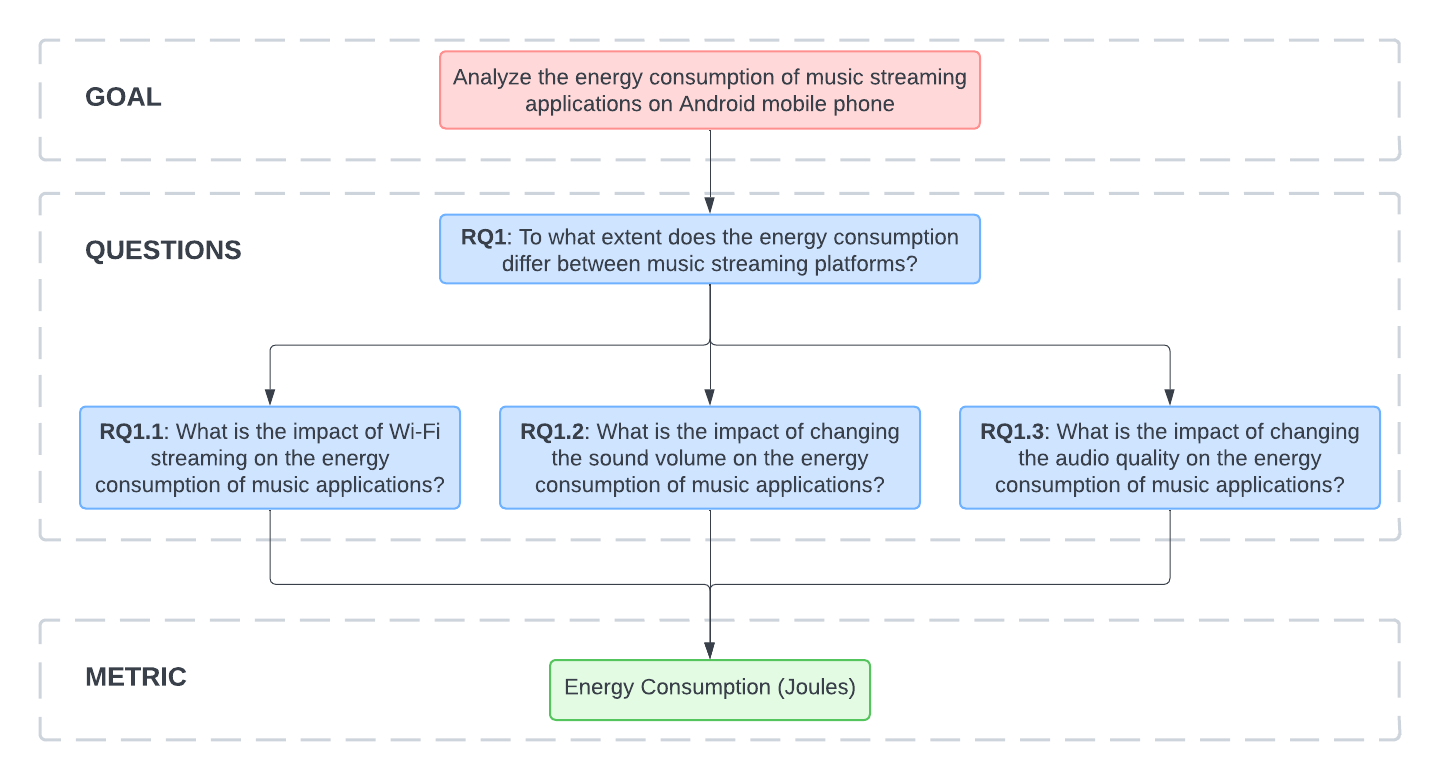
\includegraphics[width=0.8\linewidth]{figures/Visual representation of GQM.png}\textcolor{blue}{\caption{{\color{blue}Visual representation of GQM}}}
\end{figure}
\subsection{Research Questions}
To achieve the aforementioned goal, this study aims at answering one major research question (RQ1) and a set of subquestions (RQ1.1 - 1.3).

\textbf{[RQ 1]}: \emph{To what extent does the energy consumption differ between music streaming platforms?}

In general, users will be challenged by choosing from massive music players. It is not trivial for them to take energy efficiency into consideration as the battery drainage issue poses a negative impact on user experience. This question is intended to inform Android mobile devices users of the energy consumption of different music applications so that they can make a conscious decision to satisfy their requirements. 

To address this question, we compute the energy consumption of Spotify and YouTube Music based on their global popularity. According to Statista, Spotify and YouTube Music are two of the most popular music applications that recorded 13.37M and 9.42M downloads from Android users in June, 2022 \cite{13}. We subscribe to both premium versions to unlock the “very high” audio quality for later use. In order to assure the data integrity and validity, the energy consumption is measured based on a specific duration via internal speakers. Different settings are implemented as they might affect the energy consumption. We identify three possible factors that may cause sharp battery drop. They are:

1. Wi-Fi streaming vs. downloaded playing

\textcolor{blue}{2. Sound volume (\ie low, medium, and high)}

3. Audio quality (\ie , low, normal, high, and very high)

Plus,  They are formulated as sub-questions depicted below.  

  

\textbf{[RQ 1.1]}: \emph{What is the impact of Wi-Fi streaming on the energy consumption of music applications?}

In terms of saving the battery, a broad consensus is that users should avoid streaming as much as possible and play the downloaded music instead. During Wi-Fi streaming, data is exchanged over the Internet, and hence, more battery usage. It is noteworthy that both Spotify and YouTube Music store recently played songs in the cache automatically to provide buffering in case of the sudden connection error. Strictly speaking, users will not keep streaming over the same song even if it has not been downloaded yet. That is to say, Wi-Fi streaming only works the first time the user plays the song. In order to rule out the potential impact that cache might have, we compare the energy consumption caused by Wi-Fi streaming with cache cleared and downloaded file playing. 


{\color{blue}\textbf{[RQ 1.2]}: \emph{What is the impact of changing the sound volume on the energy consumption of music applications?}

Volume is decided by the amplitude of a wave, which further depends on how much energy is transferred. A speaker converts electrical energy to mechanical energy to move air to produce sound waves. The louder the sound, the more electrical energy to put in. Android devices usually have sixteen volume levels ranging from 0 (\ie mute) to 15. We select level 1, level 8, and level 15 as low, medium, and high.}

\textbf{[RQ 1.3]}: \emph{What is the impact of changing the audio quality on the energy consumption of music applications?}

 It is noticeable that the energy consumption varies based on the audio quality because the higher the quality the more data it will use up. Accordingly, frequent data transmission leads to more battery usage. {\color{blue}Both applications provide four kinds of audio quality: low, normal, high, and very high for Spotify whereas low, normal, high, always high for YouTube Music. The default audio quality settings of both applications are normal. It is worth mentioning that we rule out the “high” option in YouTube Music because in this setting, the application will adjust the audio quality automatically based on Internet condition.} We switch between all options to measure the energy consumption respectively. 
 
To ensure that experiment results can be interrupted correctly and consistently, one metric Energy Consumption, measured in Joule (J), is introduced to represent the total energy consumed over the duration. 



% Report about the GQM (with figure).

% \textcolor{red}{Page limit: 2}



\section{Experiment Planning}

\subsection{Subjects Selection}
\subsection{Experimental Variables}
\subsection{Experimental Hypotheses}
\subsection{Experiment Design}
\subsection{Data Analysis}

\textcolor{red}{Page limit: 3}
  
\section{Experiment Execution}
\subsection{Experiment Setup}
This section elaborates on the technical specifications of the infrastructure including software applications and hardware devices we use to execute the experiment. 

	Figure 2 illustrates the experimental setup that constitutes two core components, they are: (1) an Android device for running two music streaming applications, and (2) the Raspberry Pi for configuring and conducting the experiment as well as collecting the data. The Android device and the Raspberry Pi are connected via USB. Communication between them is achieved by a command-line tool Android Debug Bridge (adb)\footnote{\label{note1}\href{ https://developer.android.com/studio/command-line/adb }{https://developer.android.com/studio/command-line/adb}}. 

\begin{figure}[htbp]
 \centering
 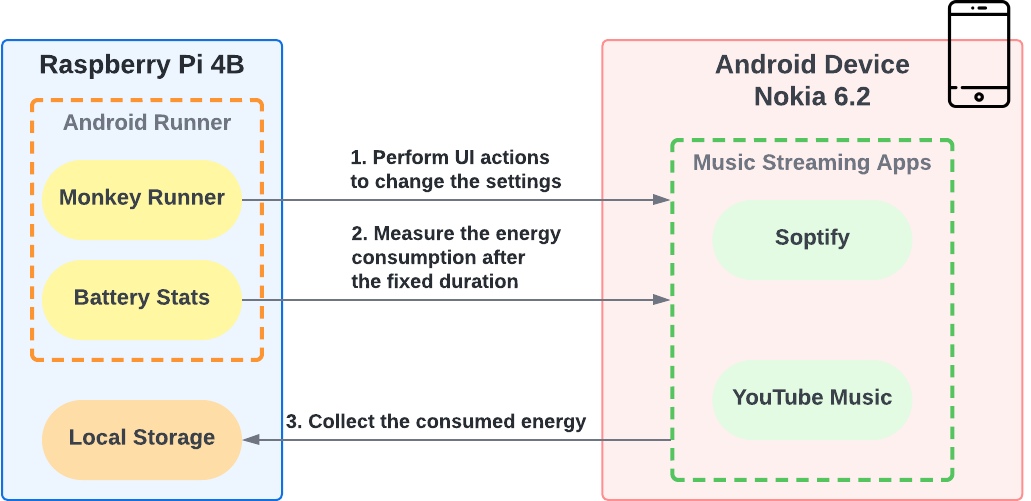
\includegraphics[width=0.8\linewidth]{figures/workflow.png}\textcolor{blue}{\caption{Experiment workflow and infrastructure}}
\end{figure}

Two music streaming applications Spotify (version 8.7.68.568, released on 22.09.2022) and YouTube Music (version 5.25.51, released on 22.09.2022) are installed from Google Play store, and run on the Nokia 6.2 mobile phone. Table 4 reports the technical specifications in detail.

Special care is taken to mitigate the effect that irrelevant factors may pose on the outcome, especially network and execution environment. On the one hand, both devices run under the same Wi-Fi network and are placed at the same distance from the router. Besides, they are the only devices that are connected to the network (if needed) during the experiment. On the other hand, the Android device is prohibited from OS updates and all third-party applications are uninstalled. 

\begin{table}[t]
\centering
\caption{Nokia 6.2 - technical specifications}
\label{table1}
\begin{tabular}{|c|c|}
\hline
CPU & 1.8 GHz Qualcomm Kryo 260 Octa-core\\
\hline

Memory & 4GB \\ 
\hline

Disk space &  64GB \\
\hline

Battery capacity &  3500 mAh \\
\hline

Screen &  6.3 inch, FHD+ \\
\hline

OS & Android 10.0 \\
\hline

\end{tabular}
\label{table_MAP}
\end{table}


In order to automate the experiment, we take advantage of the Python framework Android Runner\footnote{\label{note1}\href{ https://github.com/S2-group/android-runner }{https://github.com/S2-group/android-runner}}. We leverage an Android testing tool MonkeyRunner\footnote{\label{note1}\href{ https://developer.android.com/studio/test/monkeyrunner  }{https://developer.android.com/studio/test/monkeyrunner }} to have full control over the experiment execution. Specifically, Monkeyrunner is able to record a sequence of UI events and then replay them per request. In accordance with Android Runner, the experiment configuration is documented in JSON files that instruct Android Runner to run the experiment. Additionally, among all plugins that are integrated into Android Runner, we utilize Batterystats\footnote{\label{note1}\href{ https://github.com/S2-group/android-runner/tree/master/AndroidRunner/Plugins/batterystats}{\url{https://github.com/S2-group/android-runner/tree/master/AndroidRunner/Plugins/batterystats}}} to estimate the energy consumption in each run. 

All statistical tests are performed on RStudio\footnote{\label{note1}\href{ https://www.rstudio.com/products/rstudio/download/    }{https://www.rstudio.com/products/rstudio/download/ }} (version 4.1.2 released on 11.2021). R packages ggplot2\footnote{\label{note1}\href{ https://ggplot2.tidyverse.org/   }{https://ggplot2.tidyverse.org/}} is used for data visualization whereas effectsize\footnote{\label{note1}\href{  https://cran.r-project.org/web/packages/effectsize/index.html    }{ https://cran.r-project.org/web/packages/effectsize/index.html }} is for calculating the effect size. 

\subsection{Experiment Workflow}
To begin with, the Python script is executed to initialize an instance of Android Runner that is related to the corresponding configuration file. During one run, each instance launches the application, and sequentially alters the settings to match the current treatment parameters. Next, the Batterystats profiler comes into play. It records the energy consumption during the three minutes trial, after which Android Runner shuts down the application, followed by a one minute cooldown period. 

Precautions are taken to reduce the intrinsic variability of energy measurement. First of all, each measurement is repeated 30 times. Secondly, the execution order of each treatment is randomized. Plus, a one minute idle time is added between each run to avoid tail energy usage where certain hardware components are kept active by the operating system to lower startup energy costs \cite{li2013calculating}. Finally, cache is cleared before each run to enforce the streaming in the Wi-Fi environment. 

\href{https://docs.google.com/spreadsheets/d/1w2QG47_3Y9-IXbPPSM2fw1bH0ZvWMfadzRdfwqmWBtI/edit?usp=sharing}{\textbf{Time Log}} 
\section{Results}
Provide:
\begin{itemize}
\item descriptive statistics
\item hypothesis testing
\end{itemize}
Provide suitable plots and tables to illustrate your results.

\textcolor{red}{Page limit: Open - go deep as you wish}
\section{Discussion}
In this section, we answer all research questions on the strength of statistical tests and data analysis. In addition, we derive a list of potential factors in the music streaming application that could drain the battery. 

\textbf{[RQ 1.1]}: \emph{To what extent does the energy consumption differ between music streaming platforms?
}

The observation for RQ1 is the presence of a statistically significant difference with large effect size between Spotify and YouTube Music. To be specific, Spotify with 17.2\% less energy consumption is considered more energy-efficient than YouTube Music. As a consequence, for users who pay attention to the energy efficency, Spotify is more appealing. However, apart from energy efficiency, it is hard to argue against YouTube Music with regard to free features, audio quality, subscription, and so on. 

\textbf{[RQ 1.1]}: \emph{What is the impact of Wi-Fi streaming on the energy consumption of music applications?
}

The conclusions for RQ1.1 vary from applications. For Spotify, the null hypothesis can be rejected and we have enough evidence to confirm that connection type makes a difference on the energy consumption. Compared to Wi-Fi streaming, downloading music for offline listening leads to 2\% energy savings, which complements the small effect size. But for YouTube Music, the conclusion is just the opposite. We cannot reject the null hypothesis, and instead it can be claimed that the difference between pre-download listening and Wi-Fi streaming is minor, coupled with negligible effect size. Although Wi-Fi streaming consumes more energy to maintain an active wireless connection, it only stands out with respect to a long period. For example, previous study reports that streaming over a strong Wi-Fi connection for two hours costs a 10\% battery drop, which is twice as much as the local playing \cite{32}. The duration in each run is set to 3 minutes, so the variation of energy consumption may not be obvious enough. However, further investigation must be carried out to verify this assumption. 

\textbf{[RQ 1.2]}: \emph{What is the impact of changing the sound volume on the energy consumption of music applications?}

Similar to the two-faced conclusions for RQ1.1, applying different volume levels in Spotify leads to distinct energy consumption whereas YouTube Music does not show the relationship between sound volume and energy consumption. Nethertheless, the effect size for both applications is small. What’s more, we only observe a significant difference between low and high volume levels in Spotify. We conjecture that consumption does not vary dramatically when ranging from low to medium or medium to high level. This implication is supported by related researches, but quantitative analysis is required to provide evidence on it \cite{33}. 

\textbf{[RQ 1.3]}: \emph{What is the impact of changing the audio quality on the energy consumption of music applications?}

Changing the audio quality by far has the greatest impact on the energy consumption for both applications with great effect size. As presented in our findings, all audio qualities in YouTube have a significantly important influence on energy consumption while only very high quality in Spotify makes a difference. This could be possible due to the fact that music streaming platforms do not comply with the same audio quality classification standards. On the one hand, Spotify offers 24kbps (low), 96kbps (normal), 160kbps (high), and 320kbps (very high) audio quality, respectively \footnote{\label{note1}\href{ https://support.spotify.com/us/article/audio-quality/}{\url{https://support.spotify.com/us/article/audio-quality/}}}. On the other hand, available options in YouTube Music are 48kbps (low), 128kbps (normal), and 256kbps (always high)\footnote{\label{note1}\href{ https://support.google.com/youtubemusic/answer/9076559?hl=en}{\url{https://support.google.com/youtubemusic/answer/9076559?hl=en}}}. In general, the growth of audio quality in YouTube Music is more obvious than the one in Spotify with only one exception (\ie very high quality). There might be a threshold to determine whether the variance of different audio qualities could cause extra overhead to the Android system. Future study is needed to look into the exact cause.  


\section{Threats To Validity}\label{sec:threats}
The analysis of threats to validity is essential to acknowledge potential factors that may skew the collected data, which further determines the accuracy of the measure. It can not only facilitate the generalization of findings in similar settings but mitigate the bias in the outcome. Campbell and Cook \cite{36} proposed four kinds of threats to validity, namely internal validity, external validity, construct validity, and conclusion validity. In this section, we enumerate all threats to validity that should be taken into consideration in the context of quantitative analysis. 

\subsection{Internal Validity}
Internal validity largely relies on the extent to which alternative explanations can be eliminated. That is to say, it evaluates the rigorousness of the experiment procedure as to draw trustworthy conclusions.  

\textbf{Maturation}: This threat involves the impact of time as a variable. In particular, as time goes by, some external factors may change across trials that influence the final outcomes. It consists of temperature, file caching, and the execution order of treatments. In order to reduce the bias deriving from irrelevant factors on the results, we took numerous precautions such as randomly assigning treatments to subjects, adding a one-minute cooldown period, clearing the cache before each run, etc.  

\textbf{Reliability of Measures}: The energy consumption is solely measured by a software-based plugin Batterystats embedded in the Android ecosystem. Compared to hardware-based power profilers, software-based tools are less precise but easier to use \cite{37}. Essentially, it produces energy estimations rather than direct energy measurements. In fact, this inherent deficiency is not trivial. In the raw dataset, we observed a certain amount of identical records generated within same treatment or across different treatments, which may contribute to the substantial outliers in box plots (cf. Section 6.1). In addition, the reliability can be affected by various factors including the brightness of the mobile screen, push notifications of music streaming applications, the distance to the router, and other applications running in the background. To eliminate the influence caused by aforementioned factors, we turned off all unnecessary applications and notifications, and kept all settings the same during the experiment.   

\subsection{External Validity}

Once the internal validity has been confirmed, we move forward to the external validity, which refers to the extent to which the study results can be applied beyond the sample. 

\textbf{Interaction of Selection and Treatment}: It involves the selection of experimental subjects and the mobile device. Firstly, after leveraging the total downloads from the Google Play Store and global market share by subscribers, we narrowed down to two of the most popular Android music streaming applications Spotify and YouTube Music with caution. Therefore, benefiting from representative subjects we selected, our experiment can be replicated on other subjects, such as Amazon Music and Apple Music. Secondly, the device utilized (\ie Nokia 6.2) is a mainstream Android mobile phone with common hardware specifications. It is reasonable to assume that the experiment is conducted in a real-world scenario. 

\textbf{Interaction of Setting and Treatment}: The playing duration was fixed to 3 minutes in each run to ensure the feasibility of experiment execution and replication at the cost of realism. There is no doubt that users may not listen to music for the exact amount of time in real life. Despite the fact that the validity of duration is out of scope, this particular decision may pose a non-trivial effect on the results, especially the one related to connection type. Besides, it is widely recognized that the Internet condition is correlated to energy consumption \cite{32}. Mobile devices tend to consume more energy when connecting to a weak Wi-Fi signal. In order to mitigate this threat, the whole experiment was run under the same Wi-Fi network with irrelevant devices disconnected. 

\subsection{Construct Validity}
Construct validity refers to the extent to which the design test measures the intended construct. 

\textbf{Definition of Constructs}: We implemented the GQM framework \cite{wohlin2012experimentation} to document the experiment settings in a systematic manner. We first identified the research goal, and came up with one major research question, which was split into a set of sub-questions, followed by a common metric to answer questions. Next, the GQM-tree was formalized based on GQM components. Furthermore, we formulated null and alternative hypotheses, employed appropriate statistical tests plus effect size estimation methods. 

\textbf{Mono-method Bias}: This threat involving the dependent variable (\ie energy consumption) is complementary to the reliability of measures in the internal validity. As explained before, it is possible that Batterystats may generate less accurate measurements. However, as a widely used open source power profiler in the Android system, it has been validated and accepted by the community \cite{39}.     

\subsection{Conclusion Validity}
Conclusion validity represents the soundness of the experimental conclusion. 

\textbf{Low Statistical Power}: The cure for this type of threat is to ensure the sample size is large enough to reduce the bias as much as possible. Our study includes 2 music streaming applications with 17 treatments in total (9 treatments for Spotify and 8 treatments for YouTube Music). Each treatment is repeated 30 times with a fixed time period of 4 minutes (three-minutes execution and one-minute cooldown), adding up to 34 hours. The whole dataset constitutes 1,260 data points, which can be considered as high statistical power.

\textbf{Violated Assumptions for Tests}: Before performing statistical tests, we checked the data normality to choose between parametric and nonparametric tests which retain different assumptions. It largely reduces the possibility to draw incorrect conclusions.

\textbf{Reliability of Treatment Implementation}: In order to mitigate this threat, all treatments were designed in such a way that all of them are acknowledged as potential factors that may affect the energy consumption. 




\section{Conclusions}\label{sec:conclusions}

In this research we conducted an empirical experiment to measure the energy consumption of two music streaming applications Spotify and YouTube Music on the Android mobile device. Apart from the general comparison of energy consumed per app, we analyzed three energy-consuming factors to see if they have significant impacts on the energy consumption, namely: (1) connection type (\ie Wi-Fi streaming vs. downloaded file playing), (2) sound volume (\ie low, medium, and high), and (3) audio quality (\ie low, normal, high, very high). Our findings reveal that the energy consumption of Spotify significantly differentiates from YouTube Music with 17.2\% energy savings. In particular, the connection type influences the energy consumption in Spotify whereas the difference is minor in YouTube Music. Despite the significant impact on the consumed energy in Spotify, we deemed sound volume as a negligible issue, especially the low and the medium level. Lastly, audio quality is the dominant factor among all three to induce higher energy consumption for both applications. To summarize, this study provides guidance for users to extend their battery life and optimize towards energy consumption by adopting offline listening and avoiding high volume level and high audio quality.

The limitations of this research create opportunities for future study. Given the fact that the relatively short duration in each run may undermine the accuracy of energy estimation, we are planning to replicate the experiment with an extended time period of 10 minutes. Also, it should involve more music streaming applications to achieve better generalization. What’s more, other well-recognized energy-demanding factors like applications running as a foreground or background activity should be taken into consideration. It is a typical scenario that users have the music application running in the background with the screen locked. However, activating the app is expected to consume more energy due to the increasing uptime.

Finally, the replicated package is available for reproduction of our research as well as further investigation. 

\href{https://docs.google.com/spreadsheets/d/1w2QG47_3Y9-IXbPPSM2fw1bH0ZvWMfadzRdfwqmWBtI/edit?usp=sharing}{\textbf{Time Log}} 

\bibliographystyle{IEEEtran}
\bibliography{references}

\end{document}
